\documentclass[border=3pt]{standalone}
\usepackage{lmodern}
\usepackage{amsmath,amsfonts,amssymb}
\usepackage{pgfplots}
\pgfplotsset{compat=1.18}
\pgfplotsset{every axis/.append style={scaled y ticks=false, yticklabel style={/pgf/number format/.cd, fixed, precision=2, /tikz/.cd}}}
\usepackage{tikz}
\usetikzlibrary{arrows.meta, positioning, shapes.geometric, patterns}
\usepackage{xcolor}
\definecolor{okBlue}{RGB}{0,114,178}
\definecolor{okOrange}{RGB}{230,159,0}
\definecolor{okGreen}{RGB}{0,158,115}
\definecolor{okVermillion}{RGB}{213,94,0}
\definecolor{okPurple}{RGB}{204,121,167}
\definecolor{okSky}{RGB}{86,180,233}
\definecolor{okYellow}{RGB}{240,228,66}
\definecolor{okGray}{RGB}{120,120,120}
\begin{document}
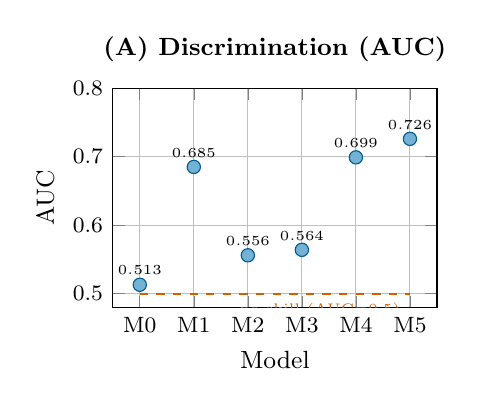
\begin{tikzpicture}
\begin{axis}[
    width=0.47\textwidth, height=0.36\textwidth,
    symbolic x coords={M0,M1,M2,M3,M4,M5}, xtick=data, ymin=0.48, ymax=0.80, ytick={0.5,0.6,0.7,0.8},
    ylabel={AUC}, xlabel={Model}, grid=both,
    tick label style={font=\footnotesize}, label style={font=\small},
    title={(A) Discrimination (AUC)}, title style={font=\small\bfseries},
    nodes near coords, every node near coord/.append style={font=\tiny, anchor=south},
    nodes near coords style={/pgf/number format/.cd, fixed, precision=3}]
\draw[dashed, thick, draw=okVermillion] ({axis cs:M0,0.5}) -- ({axis cs:M5,0.5});
\node[anchor=north east, font=\tiny, text=okVermillion] at (axis cs:M5,0.5) {no-skill (AUC$=$0.5)};
\addplot[only marks, mark=*, mark size=2.4pt, draw=okBlue!80!black, fill=okBlue!55] coordinates {(M0,0.513)(M1,0.685)(M2,0.556)(M3,0.564)(M4,0.699)(M5,0.726)};
\end{axis}
\end{tikzpicture}\hfill
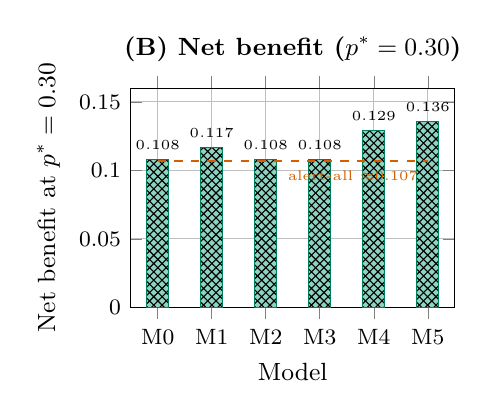
\begin{tikzpicture}
\begin{axis}[
    width=0.47\textwidth, height=0.36\textwidth, ybar, bar width=8pt,
    symbolic x coords={M0,M1,M2,M3,M4,M5}, xtick=data, ymin=0, ymax=0.16, ytick={0,0.05,0.10,0.15},
    ylabel={Net benefit at $p^*=0.30$}, xlabel={Model}, grid=both,
    tick label style={font=\footnotesize}, label style={font=\small},
    title={(B) Net benefit ($p^*=0.30$)}, title style={font=\small\bfseries},
    nodes near coords, every node near coord/.append style={font=\tiny},
    nodes near coords style={/pgf/number format/.cd, fixed, precision=3}]
\addplot[fill=okGreen!45, draw=okGreen!80!black, postaction={pattern=crosshatch}] coordinates {(M0,0.108)(M1,0.117)(M2,0.108)(M3,0.108)(M4,0.129)(M5,0.136)};
\draw[dashed, thick, draw=okVermillion] ({axis cs:M0,0.107}) -- ({axis cs:M5,0.107});
\node[anchor=north east, font=\tiny, text=okVermillion] at (axis cs:M5,0.107) {alert-all $\approx$0.107};
\end{axis}
\end{tikzpicture}
\end{document}
